\documentclass[11pt]{article}
\usepackage{deauthor}
\usepackage{times}
\usepackage{graphicx}
\usepackage{xspace}
\usepackage[square,numbers]{natbib}
\usepackage{wrapfig}
\usepackage[it,small]{caption}
\usepackage[export]{adjustbox}


\newenvironment{denselist}{
    \begin{list}{\small{$\bullet$}}%
    {\setlength{\itemsep}{0ex} \setlength{\topsep}{0ex}
    \setlength{\parsep}{0pt} \setlength{\itemindent}{0pt}
    \setlength{\leftmargin}{1.5em}
    \setlength{\partopsep}{0pt}}}%
    {\end{list}}

\newcommand{\squishlist}{
   \begin{list}{$\bullet$}
    { \setlength{\itemsep}{0pt}
      \setlength{\parsep}{2pt}
      \setlength{\topsep}{0pt}
      \setlength{\partopsep}{0pt}
      \leftmargin=25pt
\rightmargin=0pt
\labelsep=5pt
\labelwidth=10pt
\itemindent=0pt
\listparindent=0pt
\itemsep=\parsep
    }
}
\newcommand{\squishend}{\end{list}}

\setlength{\parindent}{0cm}
\setlength{\parskip}{2pt}
% use extensively to toggle between paper and TR
\newcommand{\eat}[1]{}
% \newcommand{\papertext}[1]{{\leavevmode\color{blue}{#1}}}
% \newcommand{\techreport}[1]{{\leavevmode\color{red}{#1}}}
\newcommand{\papertext}[1]{#1}
\newcommand{\techreport}[1]{}
\newcommand{\boldpara}[1]{\textbf{\paragraph{#1}}}
% de-facto paragraph format
\newcommand{\stitle}[1]{\par\noindent\textbf{#1}}
\newcommand{\cut}[1]{{\leavevmode\color{lightgray}{#1}}}
\newcommand{\ccut}[1]{} %confirmed cut
\def\plainauthor{Doris Jung-Lin Lee, Aditya Parameswaran}
\def\emptyauthor{} 
\def\plainkeywords{Data visualization, exploratory data analysis, visual querying.}
\def\plaingeneralterms{Documentation, Standardization}

\newcommand{\zv}{\textsc{Zenvisage}\xspace}
\newcommand{\vida}{\textsc{VIDA}\xspace}
\newcommand{\vidaql}{\textsc{VIDA-QL}\xspace}
\newcommand{\sbd}{\textsc{Storyboard}\xspace}
\newcommand{\ssearch}{\textsc{ShapeSearch}\xspace}
\newcommand{\seedb}{\textsc{SeeDB}\xspace}

\newcommand\notes[1]{\textcolor{red}{#1}}

% To make various LaTeX processors do the right thing with page size.
\def\pprw{8.5in}
\def\pprh{11in}
\special{papersize=\pprw,\pprh}
\setlength{\paperwidth}{\pprw}
\setlength{\paperheight}{\pprh}
\setlength{\pdfpagewidth}{\pprw}
\setlength{\pdfpageheight}{\pprh}
%%%%%%%%%%%%%%%%%%%%%%%%%%%%%%%%%%%%%%%%%%%%

\begin{document}
\title{The Case for a {\em Visual Discovery Assistant}: \\ A Holistic Solution for Accelerating Visual Data Exploration}

\author{\plainauthor\\
\{jlee782,adityagp\}@illinois.edu\\
University of Illinois, Urbana-Champaign}
\maketitle
\begin{abstract}
Visualization is one of the 
most effective and widely-used 
techniques for understanding data. 
Yet, the growing use of visualizations 
for exploratory data analysis 
poses new demands beyond simply 
the graphical presentation 
and visualization authoring 
capabilities offered in existing tools. 
In particular, many data analysis
tasks involve navigating large 
collections of visualizations to make sense
of trends in data;
at present, this navigation is done manually or
programmatically. 
We outline a vision for an
intelligent, interactive, understandable,
and usable tool 
that can help automate
this largely manual navigation: we call our tool \vida\footnote{Vida means {\em life} in Spanish.}---short for {VIsual Discovery Assistant}. 
We argue that typical navigation tasks can be 
organized across two dimensions---overall goal 
and precision of specification.
We organize prior work---both our own work, as well
as other ongoing work in this area---across 
these two dimensions, and highlight
new research challenges.
Together, addressing these challenges underlying \vida
can help pave the way for a comprehensive
solution for removing the pain points
in visual data exploration.
\end{abstract}


\section{Introduction}% 
\par With the ever-increasing complexity 
and size of datasets,
there is a growing demand for 
information visualization tools
that can help data scientists make sense of large
volumes of data.
Visualizations help discover 
trends and patterns, 
spot outliers and anomalies, 
and generate or verify hypotheses.
Moreover, 
visualizations are accessible and intuitive: 
they tell us stories about our data; 
they educate, delight, inform, 
enthrall, amaze, and clarify.
This has led to the overwhelming popularity
of point-and-click visualization tools like Tableau~\cite{Stolte2002},
as well as programmatic toolkits like ggplot, D3, Vega, and matplotlib. 
We term these tools as {\em visualization-at-a-time} approaches, since
data scientists need to individually 
generate each visualization (via code or interactions),
and examine them, 
one at a time.


\par
As datasets grow in size and complexity, 
these visualization-at-a-time approaches start to break down,
due to the limited time availability on the 
part of the data scientists---there 
are often too many visualizations to examine for a given 
task, such as identifying outliers, or inferring patterns. 
Even on a single table, 
visualizations can be generated
by varying the subsets of data operated on, 
or the attributes (or combinations
thereof) that can be visualized. 
If we add in various visualization modalities, encodings,
aesthetics, binning methods, and transformations,
this space becomes even larger. 
(For this work, we focus primarily on
the impact of varying the data subsets
and attributes visualized---some of these
latter concerns are the focus of recent work~\cite{Wongsuphasawat2017}.)

\begin{wrapfigure}{l}{0.4\textwidth}
\centering
\vspace{-10pt}
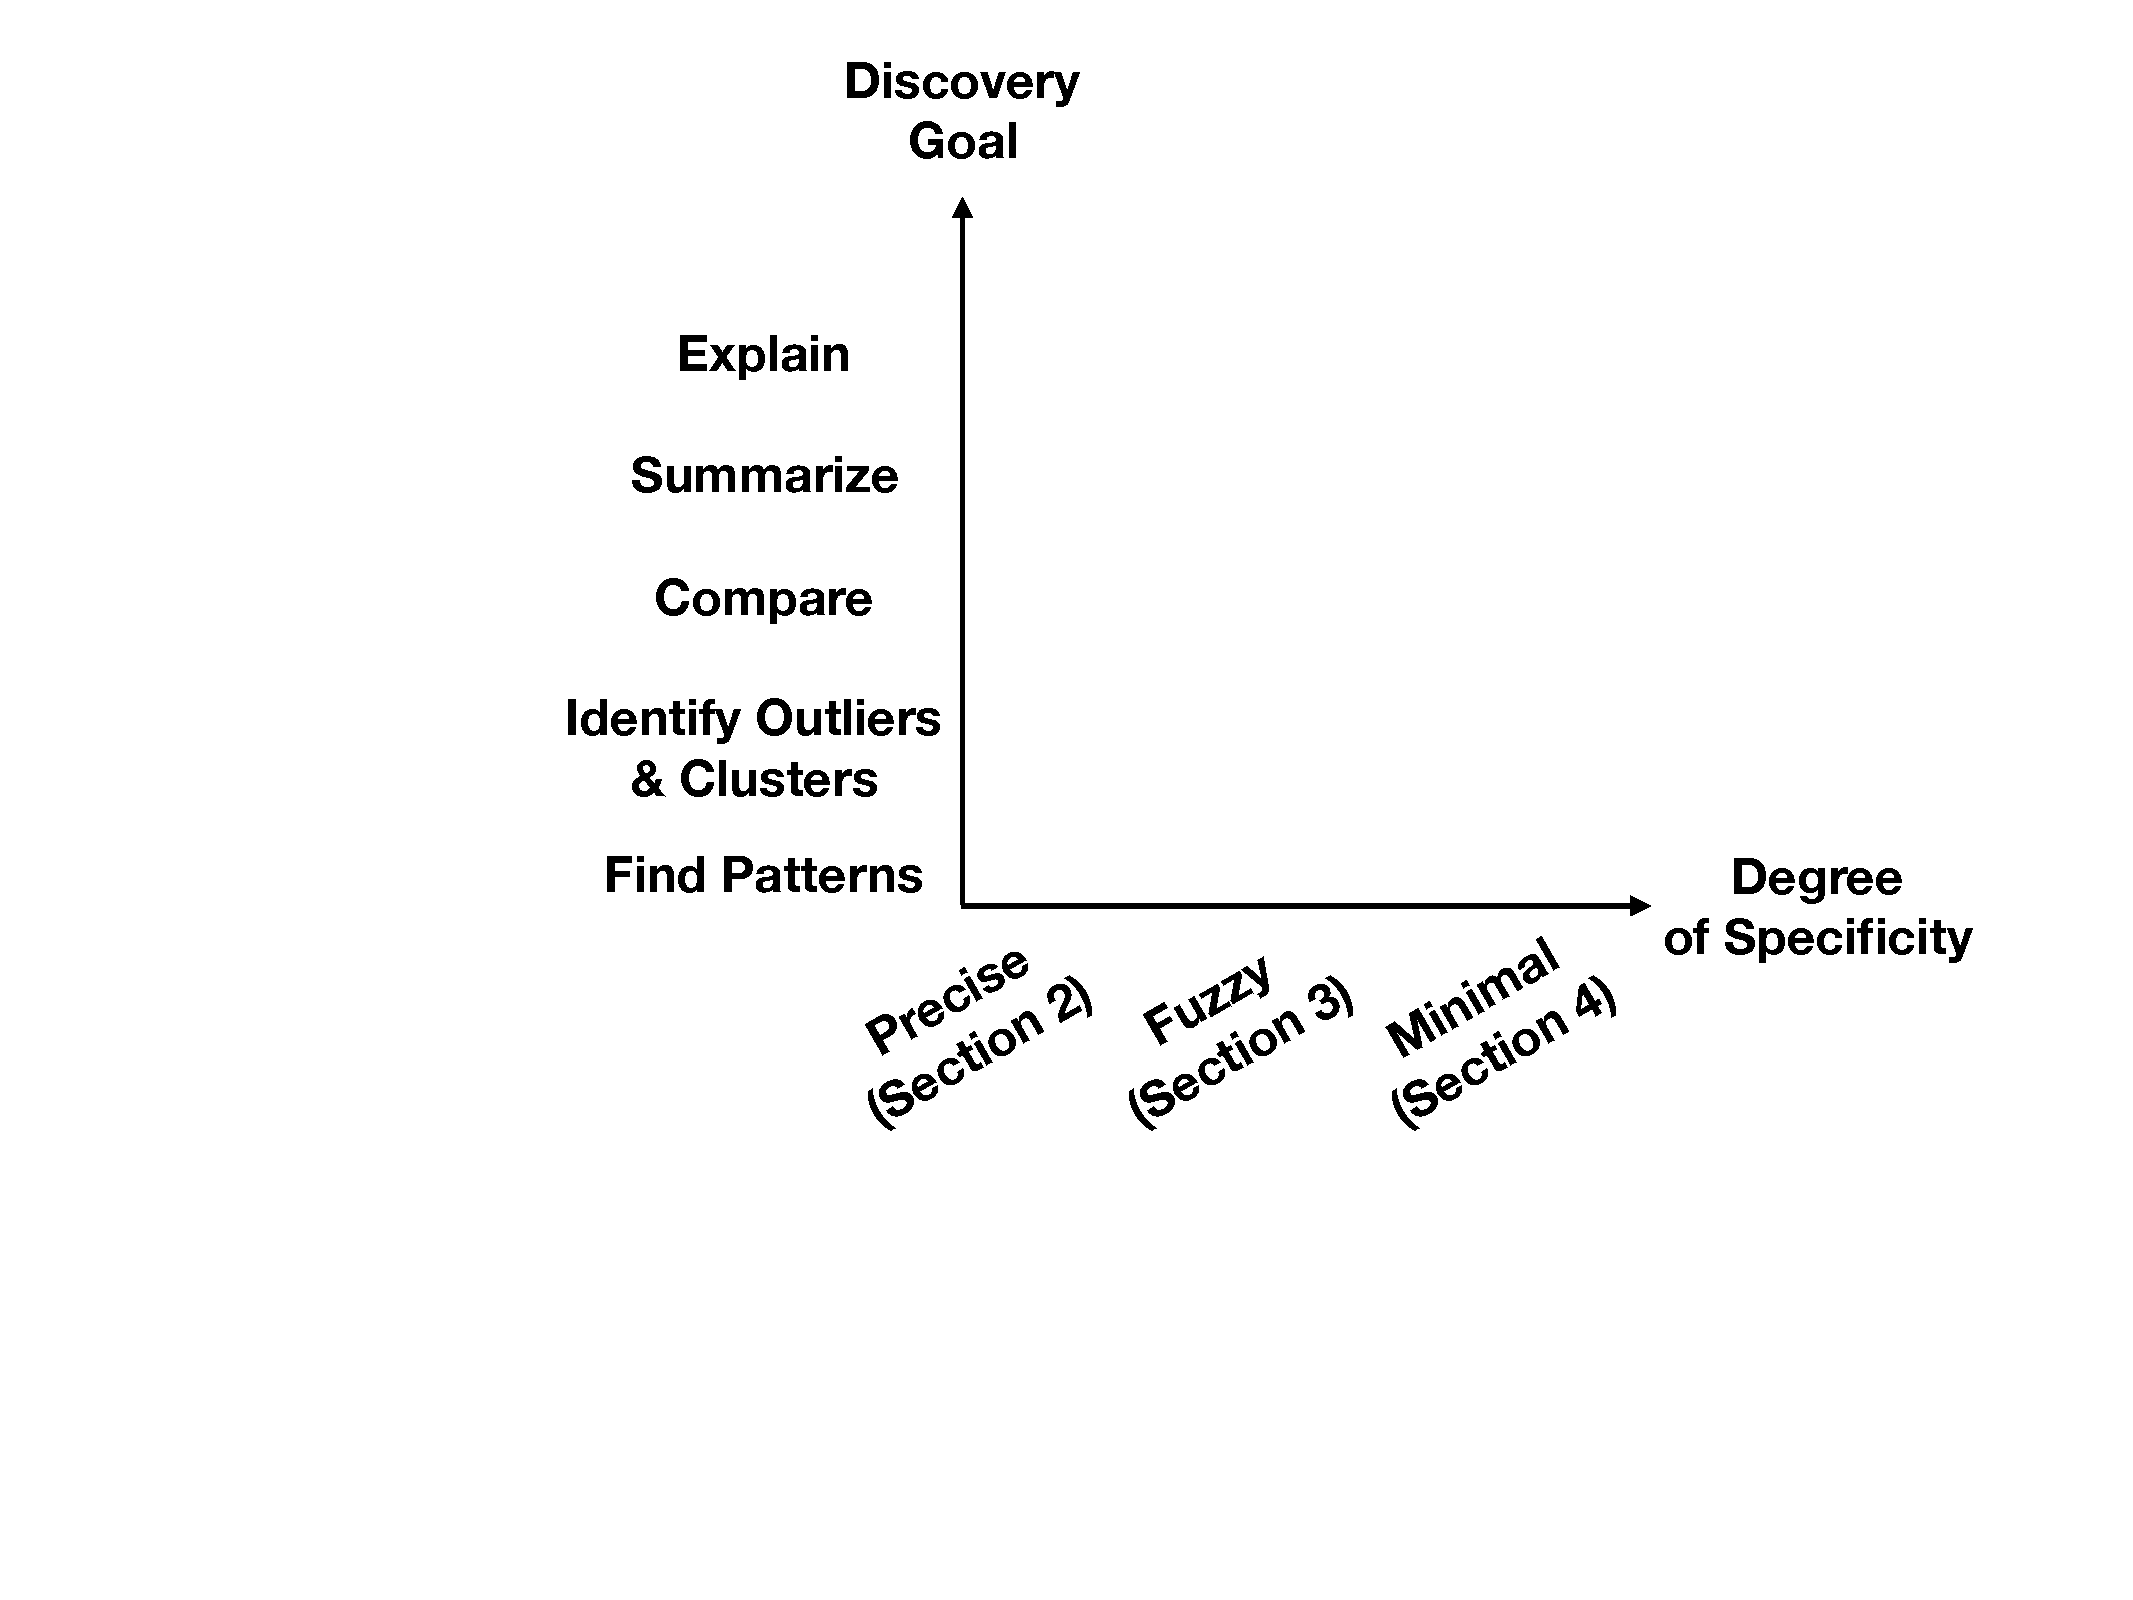
\includegraphics[width=\linewidth]{figs/dimensions.pdf}
\vspace{-15pt}
\caption{The two dimensions of discovery settings. The Y axis depicts the different discovery goals ordered in roughly increasing complexity, while the X axis characterizes decreasing levels of query specificity and correspondingly increasing levels of autonomous assistance.}\label{fig:dimensions}
\vspace{-15pt}
\end{wrapfigure}


\par Thus, there is a pressing need for an 
intelligent,
interactive, understandable, usable, and
enjoyable tool that can help 
data scientists navigate
collections of visualizations, across a range of possible analysis goals and modalities that data scientists may require.
We term our hypothesized comprehensive tool \vida,
short for {\em VIsual Discovery Assistant}.
Data scientists can specify any discovery
goal at a high level, in one of many intuitive input modalities supported in \vida, with \vida automatically traversing visualizations to provide solution or guidance for the
specified discovery goal, thereby
eliminating the tedium and wasted
labor of comparable visualization-at-a-time 
approaches.

\par \stitle{\vida Dimensions.} 
In order to be a holistic solution for 
navigating collections of visualizations,
\vida must be able to support various discovery
settings. 
We organize these settings along two
dimensions, displayed along the Y axis and 
X axis (respectively) of Figure~\ref{fig:dimensions}---first, 
the overall discovery goal,
and second, the degree of specificity of the input query.

\par Along the Y axis, we identify five 
common discovery goals in visual data exploration:
{\em finding patterns}, {\em identifying anomalies/clusters}, {\em summarizing}, 
{\em performing comparisons}, {\em providing explanations}.
These five goals borrow from functionalities in existing
systems, as well as related visualization task taxonomies~\cite{Amar2005,Heer2012}.
They are organized along the Y axis in a sequence of roughly increasing complexity; however, we must emphasize that these goals are distinct from one other. 
We omit low-level goals such as filtering or sorting, since these functionalities are common in existing visualization-at-a-time tools and toolkits. We also omit goals that go beyond visual data exploration, such as extrapolation, supervised learning, and cleaning, among others. 

\begin{wrapfigure}{r}{0.5\textwidth}
\centering
\vspace{-15pt}
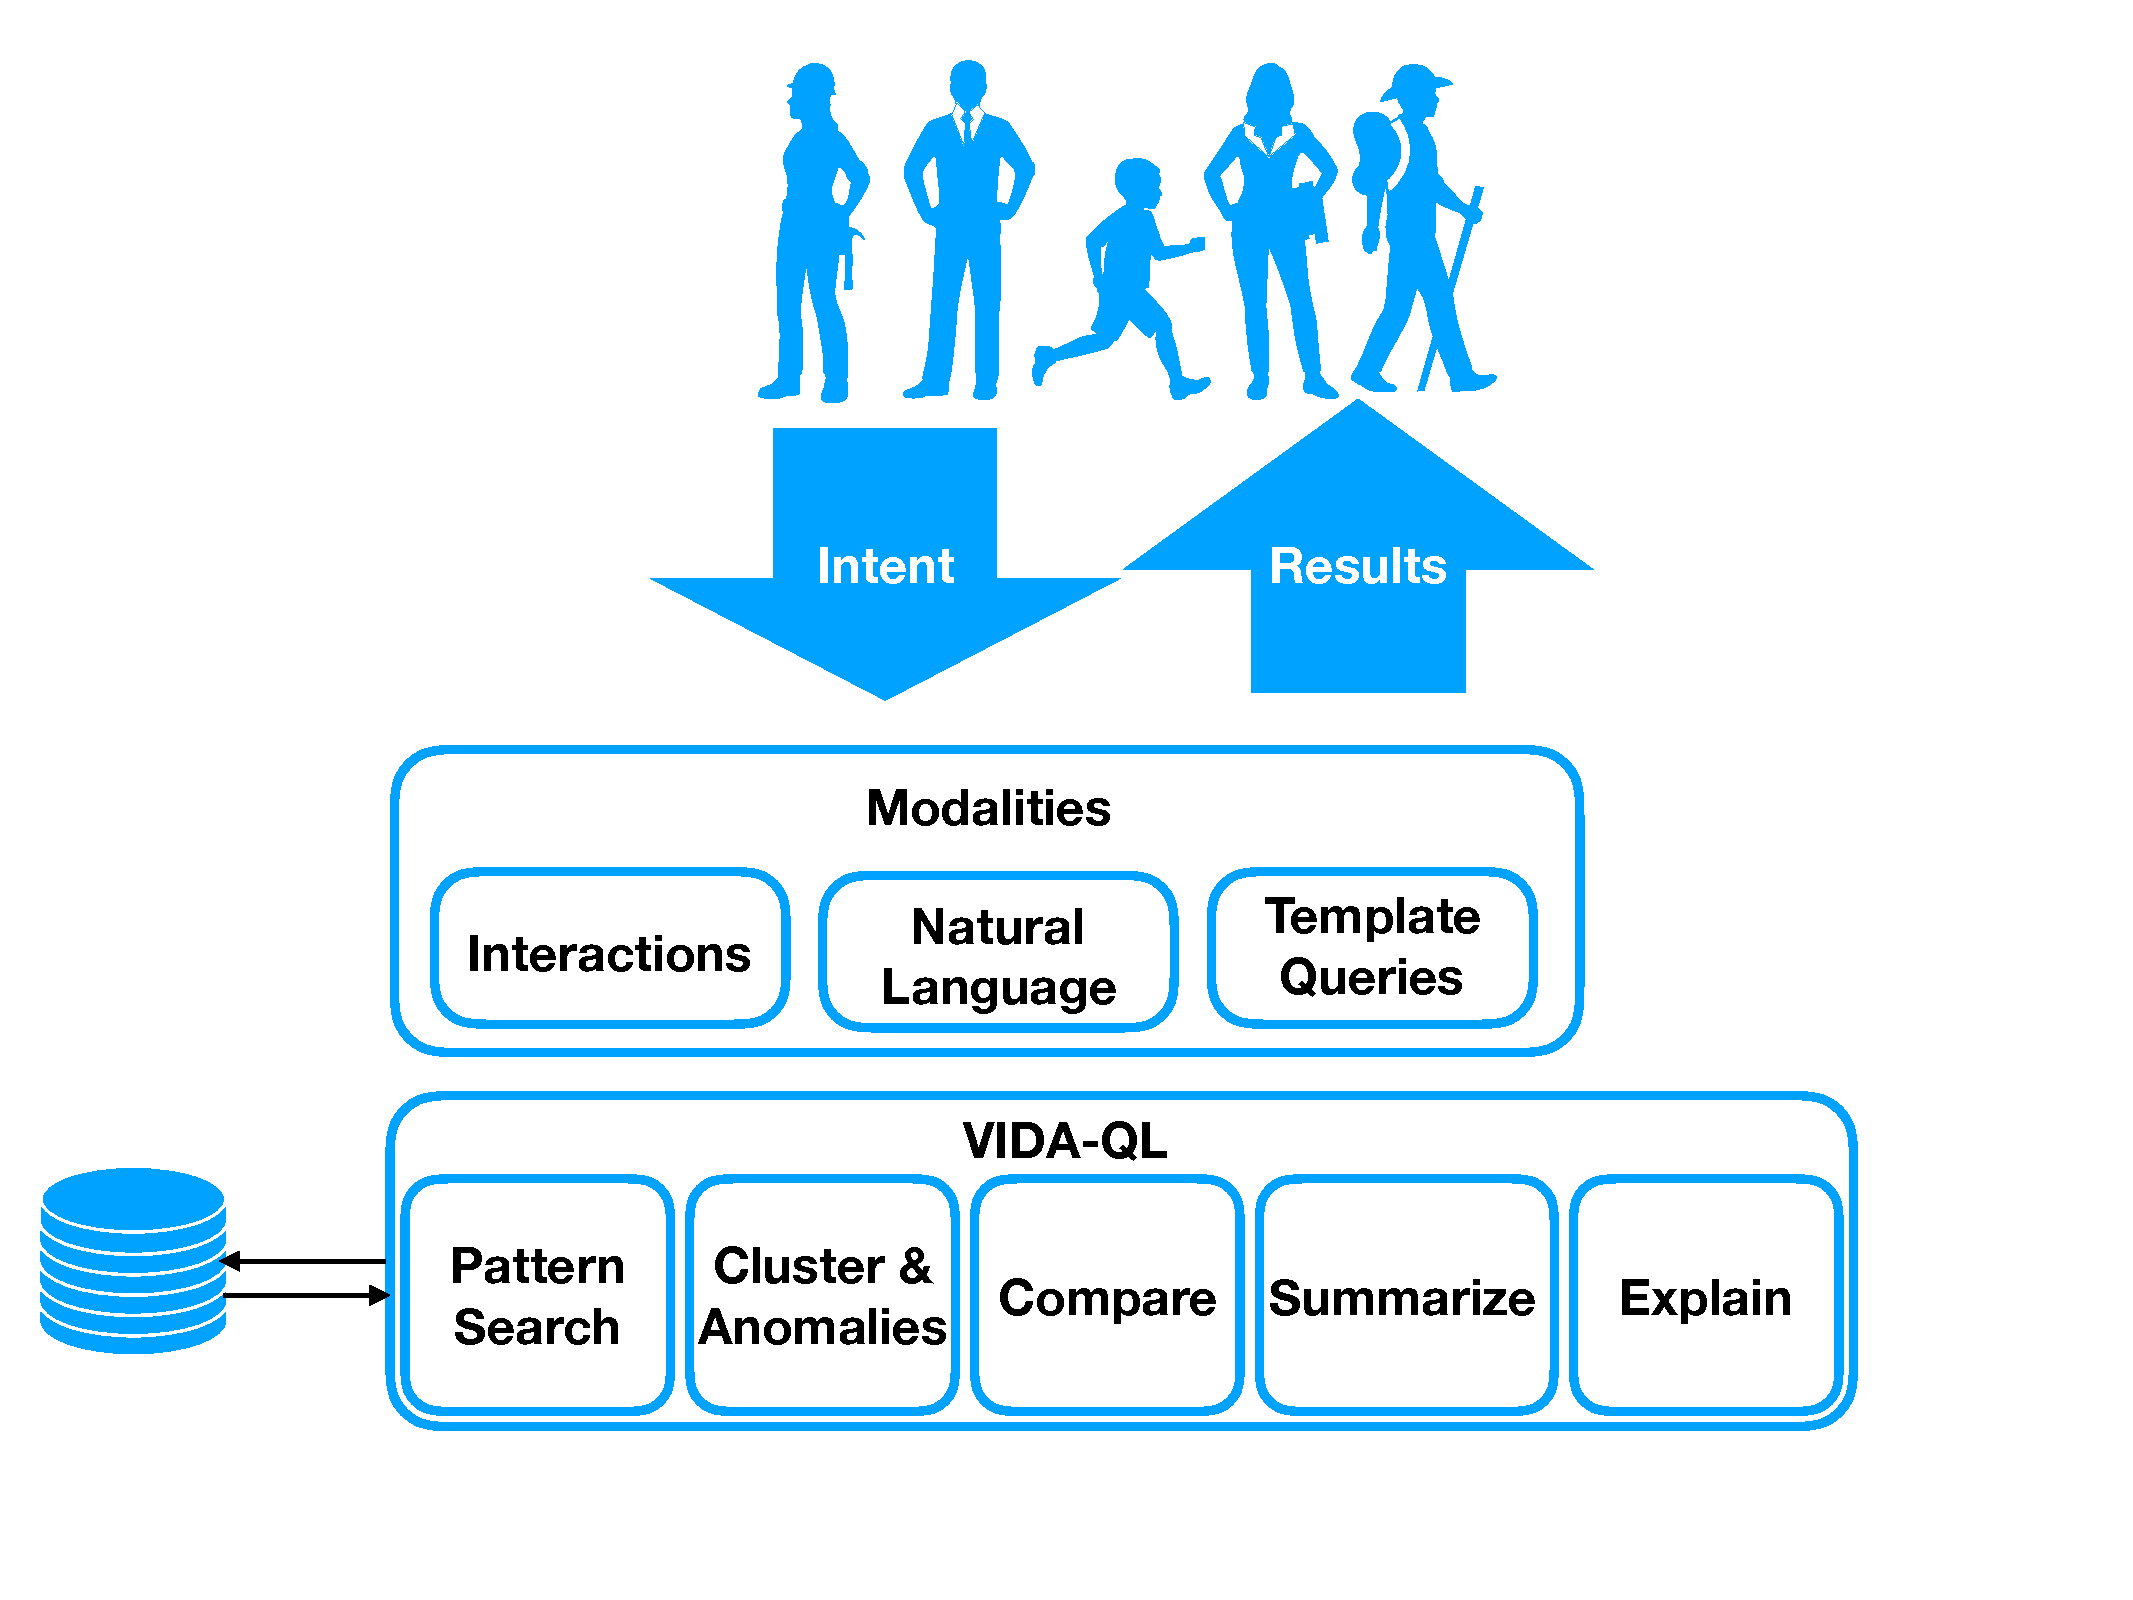
\includegraphics[width=\linewidth]{figs/VIDA_architecture.pdf}
\vspace{-25pt}
\caption{\vida Architecture\label{fig:vida_architecture}
\vspace{-15pt}
}
\end{wrapfigure}


\par 
 We identify three degrees of specificity
for the query input, organized along the X axis:
{\em precise}, {\em fuzzy}, {\em minimal}.
The degree of specificity characterizes the division
of work between how much user has to specify
versus how much the system has to automatically
infer and aid in accomplishing the discovery goal. 
For the precise setting, the onus is placed on the user
to provide an exact and complete specification of 
what the solution to their discovery
goal must look like;
for the fuzzy setting, the user can provide
a vague specification of what the solution must look like;
and finally, for the minimal setting,
the user provides a minimal specification, or
leaves the characteristics of the solution underspecified,
leaving it up to the system to ``fill in'' the rest.
As we proceed along the X axis,
it gets harder for the system to automatically
interpret what the user might have in mind as a solution
to their goal.

\par \stitle{\vida Input Modalities.} To support the spectrum of 
demands imposed by the
discovery settings described above, \vida 
must support a range of interactive input modalities,
as displayed in Figure~\ref{fig:vida_architecture},
catering to a range of user expertise and preferences.
These input modalities include: 
\squishlist
	\item restricted template queries, involving selection of operators and operands from a drop-down menu; and
	\item interactions, either with an existing visualization, such as brushing-and-linking or hovering, or those that construct a new one, such as drag-and-drop or sketching; and
	\item natural language, via a keyword search box, dialog, or conversational interface.
\squishend
Each of these inputs are compiled down
into a query in a query language, called \vidaql.
Alternatively, expert users may directly invoke \vidaql queries.
\vidaql queries will natively support the five discovery goals and combinations thereof, e.g., summarization followed by pattern search. Another important element is how much does a user actively requests for visualizations (``pull'') versus how much \vida recommends visualizations (``push''). Given that we expect \vida to support a range of specificities, \vida must support both push and pull, with pull decreasing in importance and push gaining importance, as we go from the precise to minimal setting.

\par
\stitle{Present Day Visual Query Systems.}
We have described \vida so far as if no comparable capabilities
exist today.
This is not the case; in Table~\ref{fig:table}, we list some examples of systems
that partially provide the functionality of \vida,
for certain settings and input modalities.
We will describe some of these systems later on in the paper. 
Since all of these systems allow users to query data {\em visually},
we call these systems {\em Visual Querying Systems}, or VQSs for short.
VQSs typically {\em (i)} 
employ objectives that are perceptually-aware,
taking into account for the fact that the results are typically
consumed by a human analyst, rather than an algorithm;
{\em (ii)} provide some interactive interface or declarative capabilities
to express the discovery goal as a ``what'' rather than a ``how'';
and {\em (iii)} possess optimization capabilities to facilitate
the efficient discovery of visual insights. 


\begin{table}[!t]
\scriptsize
\centering
\begin{tabular}{l|l|l|p{7.5cm}}
VQS & Discovery Goals Covered & Specificity & Interactions Supported \\ \hline

Zenvisage~\cite{Lee2017,Siddiqui2016} & Find Patterns, Cluster/Outliers, Compare & Precise & Interactions (Clicking, Sketch, Drag-and-drop), Query Language \\
TimeSearcher~\cite{hochheiser2004dynamic} & Find Patterns, Cluster/Outliers & Precise & Interactions (Clicking, Sketch) \\ 
Query-by-Sketch~\cite{wattenberg2001sketching} & Find Patterns & Precise & Interactions (Clicking, Sketch) \\ 

Scorpion~\cite{Wu2013} & Explain & Fuzzy & Interactions (Clicking) \\

ShapeSearch~\cite{Siddiqui2018} & Find Patterns & Fuzzy & Interactions (Sketch), Natural Language, Query Language \\

%Data Polygamy~\cite{chirigati2016data} & Compare, Explain & Fuzzy & Query Language \\
Profiler~\cite{Kandel2012} & Compare & Fuzzy & Interactions (Clicking, Brushing-and-Linking) \\
SeeDB~\cite{Vartak2015} & Compare & Minimal & Interactions (Clicking) \\
Storyboard~\cite{Lee2018} & Cluster/Outliers, Compare, Summarize & Minimal & Interactions (Clicking) \\
iDiff~\cite{Sarawagi1998,Sarawagi2000} & Compare, Explain & Minimal & Query Language \\

\end{tabular}
\vspace{-10pt}
\caption{A Sample of Visual Query Systems}\label{fig:table}
\vspace{-10pt}
\end{table}

\par \stitle{Outline.}
The rest of our paper is organized along the degree of specificity
of discovery goal, and we will allude to the specific discovery
goals as well as input modalities as we go along. 
The degree of input specificity is the factor
that most significantly affects the architecture of \vida,
with the complexity increasing as the specificity decreases---in that
the system has to do more ``guesswork'' to support underspecified goals. 

\par We begin by discussing the 
the {\em precise} setting (Section~\ref{sec:precise}).
We describe \zv~\cite{Siddiqui2016} 
as a partial solution for
this setting, and thereby a starting point for \vida,
partially eliminating the problem
of having to manually examine large numbers 
of visualizations for a given discovery goal, 
which can be error-prone and inefficient.

\par However, a design study using \zv demonstrates
that the precise setting is insufficient for
addressing all of the demands of real-world use-cases~\cite{Lee2017}.
In particular, users do not have
a clear understanding of their querying intent without looking at example visualizations or summaries of the data, and even when they do, their intent involves
vague or high-level notions that can not be expressed clearly.

\par To bridge the gap between the user's high-level
intent and the system demands,
we outline a set of research challenges
that goes beyond simple precise visual querying, by
(a) supporting a wider class of vague or ``fuzzy'' high-level
queries, thereby increasing the expressiveness
of \vida (Section~\ref{sec:vague});
and 
(b) making it easier to know what to query
by recommending visualizations that provide
a high-level understanding of the data (Section~\ref{sec:minimal}).

\stitle{Interfaces and Interactions, not Optimization.}
In this paper, we focus our attention on the interfaces,
query languages, and capabilities, 
and how to use them to capture discovery goals
with varying degrees of specification, as opposed to optimization.
Indeed, once the query is issued in some form 
(say, translated into a \vidaql
query),
optimization is crucial to try to traverse the space 
of visualizations and return results in an interactive manner.
A range of techniques may be adopted for this purpose,
including parallelism, multi-query optimization, sampling,
pruning, and pre-computation~\cite{Siddiqui2016,Vartak2015}.
We expect a similar combination of techniques to be applicable to
each of the settings that we consider. To limit the scope of this paper, we have
decided to avoid describing optimization aspects and focus on the interfaces and interactions instead.

%!TEX root = main.tex

\section{The Precise Setting: Existing Visual Query Systems}\label{sec:precise}
While visual data exploration often reveals 
important anomalies or trends 
in the data~\cite{Heer2012,Morton2014}, 
it is challenging to 
use visualization-at-a-time systems to 
repeatedly choose the right subsets of 
data and attributes to visualize
in order to identify desired insights.
We first motivate the precise setting through a use-case from astronomy.

\subsection{Motivating Example: Discovering Patterns in Astronomical Data}
Astronomers from the Dark Energy Survey (DES) 
are interested in finding 
anomalous time series 
in order to discover 
transients, 
i.e., objects whose brightness 
changes dramatically as a function of time, 
such as supernova explosions or quasars~\cite{Drlica-Wagner2017}. 
When trying to find celestial objects 
corresponding to supernovae, 
with a specific pattern of brightness over time, 
astronomers individually inspect the corresponding 
visualizations until 
they find ones that match the pattern. 
With more than 400 million objects in their catalog, 
each having their own set of time series brightness measurements, 
manually exploring so many 
visualizations is not only error-prone, 
but also overwhelming.
Many astronomers instead rely on guess-work 
or prior evidence to explore the visualizations,
rather than directly ``searching'' for the patterns
that they care about. 
While most astronomers do use 
programming tools, such as Python and R,
it is cumbersome to express each new information need
via carefully hand-optimized code. 
The astronomy use case highlights a 
common challenge in visual data exploration,
where there are often a large number of visualizations
for each discovery goal,
and manual exploration is impossible.
There is no systematic way to create, compare, filter,
and operate on large collections of visualizations.

\subsection{Ongoing Work and Research Challenges within the Precise Setting}

\stitle{Discovering Patterns and Anomalies/Clusters, and Performing Comparisons with \zv.}
\zv is an example of a VQS that operates on 
large collections of visualizations.
\zv is built on top of a visual query language
called ZQL, which operates on collections of visualizations, and returns
collections of visualizations,
using primitives such as visualization composition,
sorting, and filtering~\cite{Siddiqui2016}. 
In addition, via user-defined functions (also provided as built-ins),
ZQL can compute the distance for a visualization from another---and this
distance can be used as a building block for more complex
operations, such as the first three discovery goals listed
in Table~\ref{fig:table}, i.e., finding a visualization
matching a pattern, detecting an outlier or cluster centers,
or comparing visualizations with each other.
Thus, ZQL operates at a level higher than
languages for specifying visual encodings of
individual visualizations~\cite{Stolte2002,Wilkinson2005}.
ZQL can be used to construct a rich variety of queries,
including the following on a real-estate dataset:
\squishlist
	\item {\em Find Patterns.} Find visualizations of cities whose housing price over time is similar to Manhattan. 
	\item {\em Identify Anomalies.} Find visualizations of cities with both an increasing housing price trend and an increasing foreclosure rate trend.
	\item {\em Perform Comparisons.} Find visualizations for which New York and Champaign differ the most.
	\item {\em Find Patterns, followed by Clusters.} For cities that are similar
	to New York on sales price trends, find typical trends for foreclosure rates.
\squishend

\par While ZQL is a useful starting point, writing ZQL
queries can be daunting for users who are not comfortable
with programming.
Therefore, we extracted a typical workflow
of visual querying for finding patterns, identifying
outliers and clusters, and making comparisons, and made it expressible
via simple interactions. As shown in Figure~\ref{fig:modalities}, the user can input their search pattern via (a) inputting a set of points,
(b) a sketch, (c) dragging-and-dropping an existing visualization,
or (d) inputting an equation, 
and specify a space of visualizations over which to search.
The system returns a ranked list of matching visualizations, shown in the ``Results'' pane below the canvas in (b), for the corresponding ZQL query.
The system also provides typical trends 
(called ``Representative Patterns'', highlighted under (c)) and outliers
for additional context. 
The user can also switch to a tabular interface wherein
they can input ZQL queries.  
Users can also make comparisons between different 
subsets of the data by examining visualizations 
of dynamically created classes in \zv~\cite{Lee2017}.
Thus, this workflow captures one variation of the three
discovery goals---finding patterns, identifying outliers/clusters,
and making comparisons. 
\begin{figure}[!t]
\centering
\vspace{-10pt}
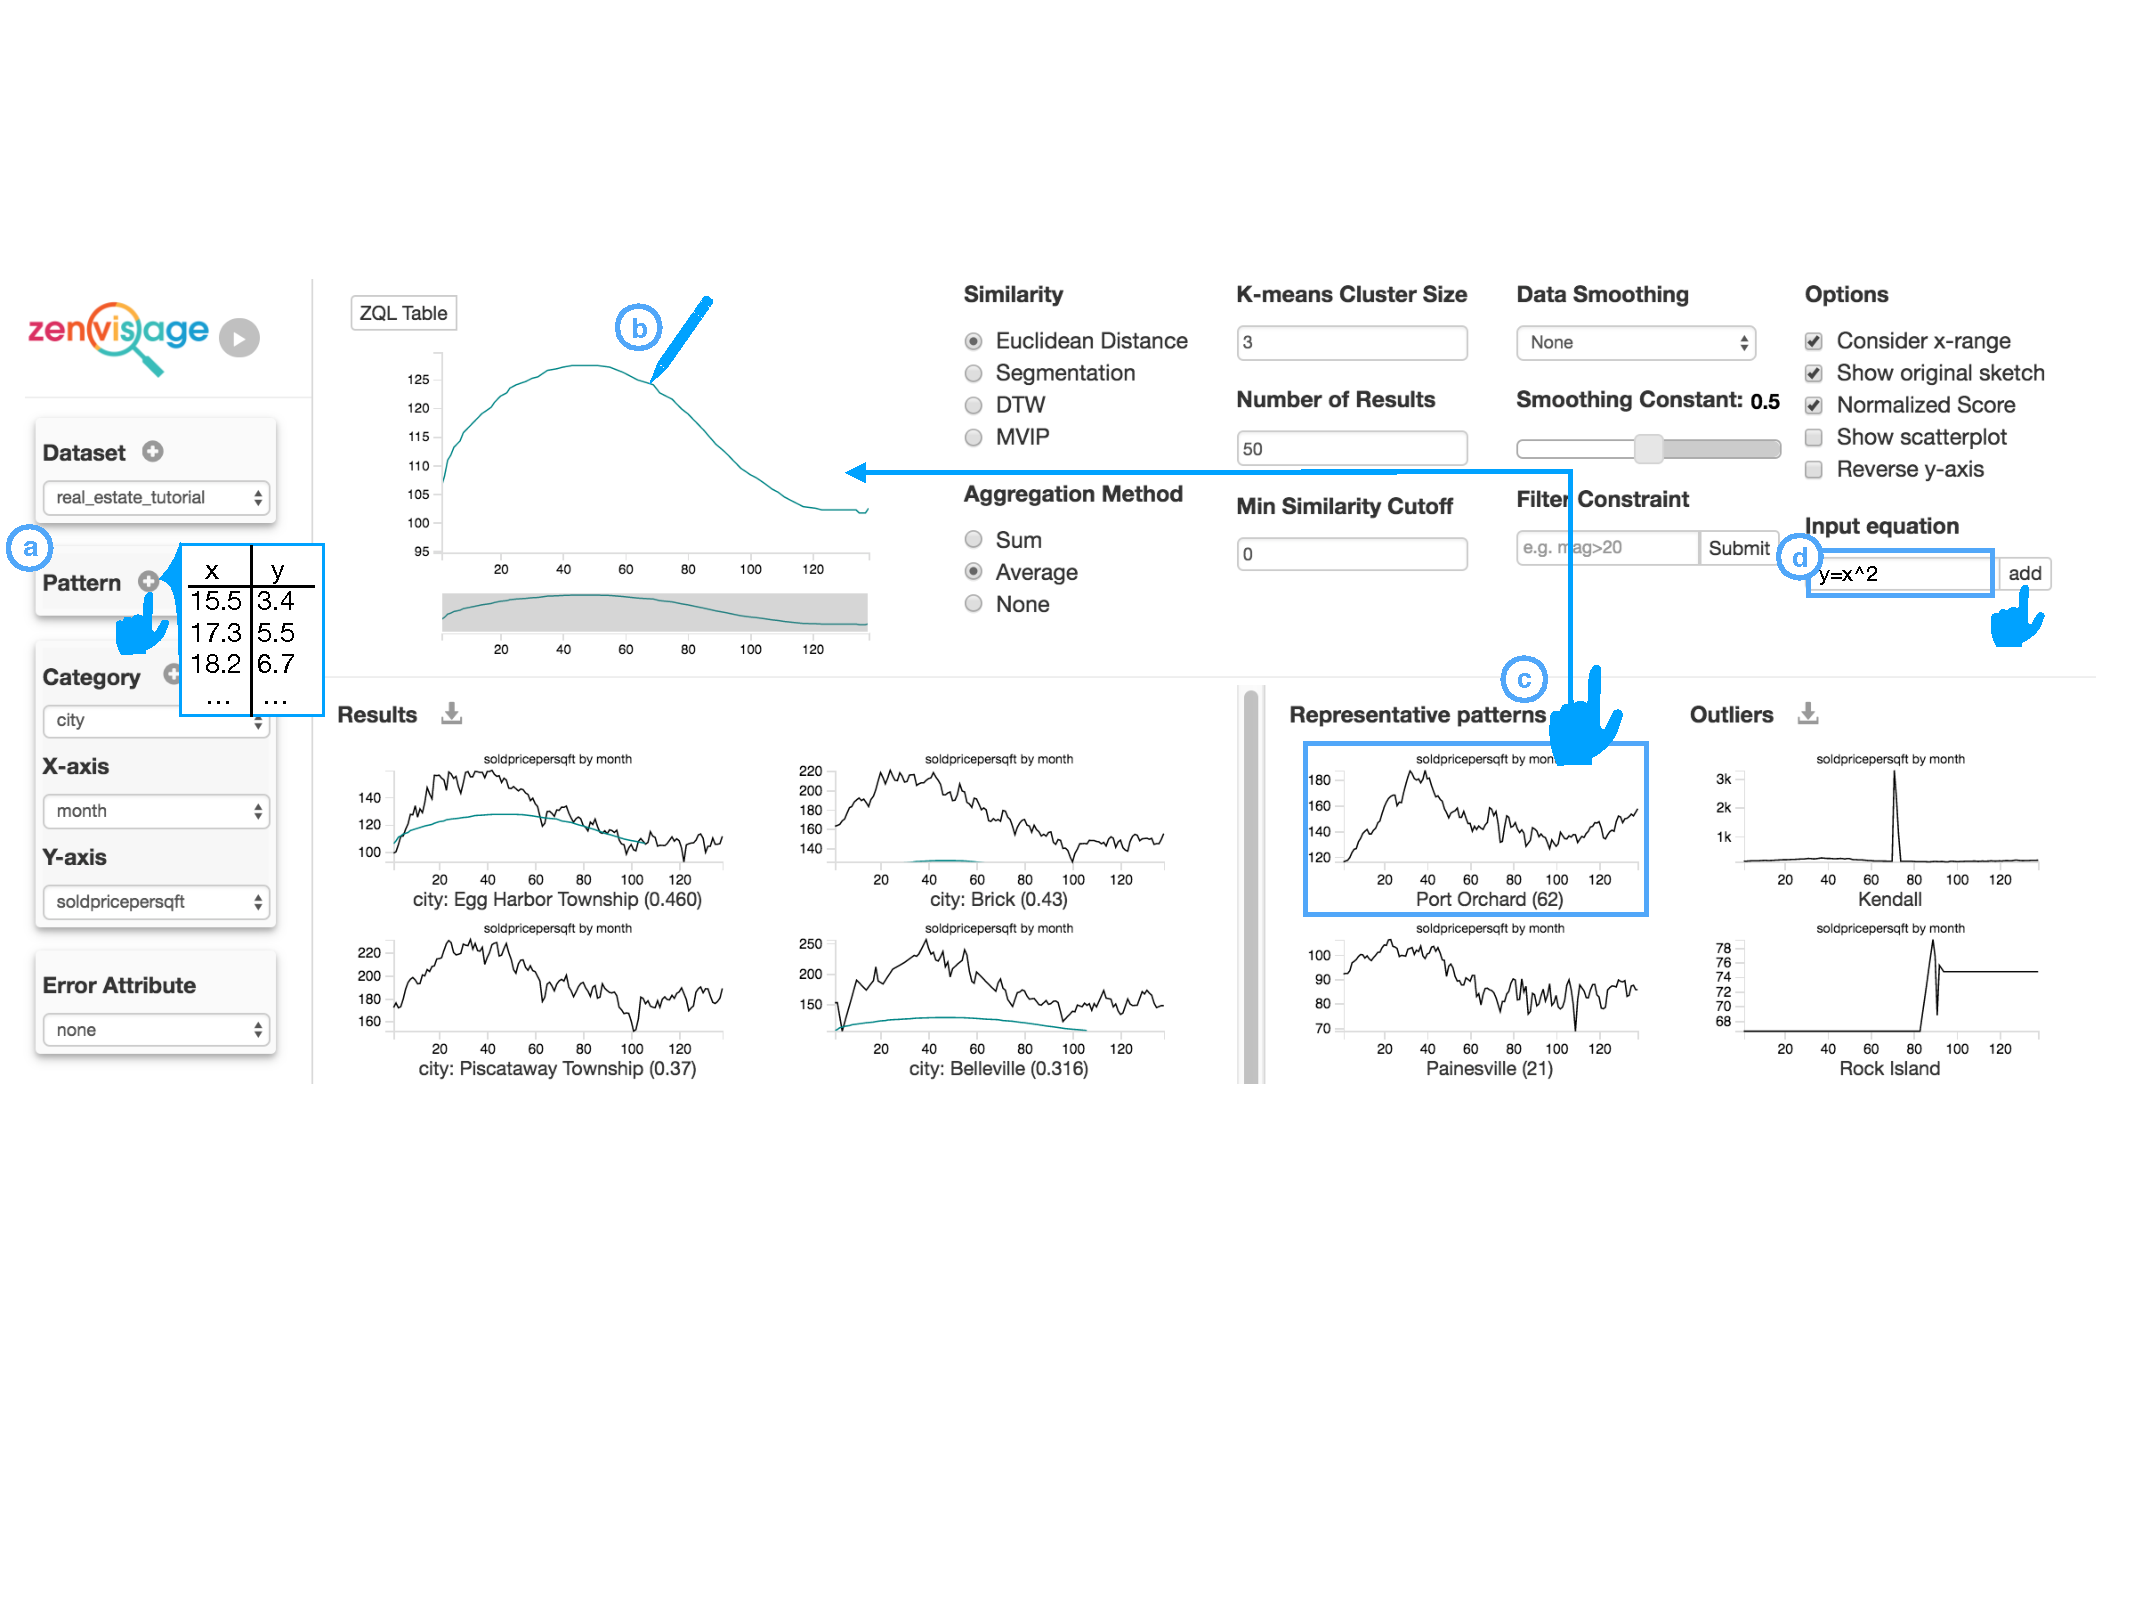
\includegraphics[width=0.8\textwidth,frame]{figs/modalities.pdf}
\caption{\zv offers a variety of querying modalities, including: a) uploading a sample pattern from an external dataset as a query, b) sketching a query pattern, c) dragging-and-dropping an existing pattern from the dataset, and d) inputting an equation as a query, from \cite{Lee2017}.}
\label{fig:modalities}
\vspace{-10pt}
\end{figure}


\stitle{Other Related Precise Visual Querying Systems.}
There has been a range of work primarily focused on locating visualizations
matching certain patterns, including the influential work
on TimeSearcher~\cite{hochheiser2004dynamic}, where the query is
specified as a box constraint, and 
Query-by-Sketch~\cite{wattenberg2001sketching}, where the query is 
sketched as a pattern. 
This was applied to search queries within Google Correlate~\cite{mohebbi2011google}. 
Recent work has also extended this to querying using regular
expressions~\cite{Zgraggen2015}, while
others have analyzed the semantics
of sketches~\cite{correll2016semantics,Mannino2018}.

\stitle{Limitations within the Precise Setting.}
The most important challenge within the precise setting
is the following: {\em How do we expose the entire capabilities of
 \vidaql via intuitive interactions and discoverable
modules?} So far, most tools that we listed above
support a restricted set of interactions,
primarily focused on finding patterns via sketches or box constraints. 
\zv extends and builds on this 
by supporting outlier and representative trend discovery
from the front-end interface. 
Unfortunately, performing comparisons, deriving explanations, or summaries,
is hard to do interactively. 
In fact, deriving explanations or summaries
is hard to do even with the full power of ZQL, since
it does not support the synthesis of new information
that goes beyond simple processing of collections of visualizations. 
It remains to be seen if and how ZQL can be extended to meet these capabilities.
Moreover, even for sketching, it would be interesting to see if
we can support analogous pattern search mechanisms
for other visualization types, such
as scatterplots
or heatmaps.


\subsection{Limitations with the Precise Setting}
\par Even if we could address 
the issues within the precise setting
in the previous section,
there are some fundamental limitations
with the precise setting itself 
that need to be addressed within a full-fledged \vida.
We discuss these limitations
in the context of a participatory 
design process for the development 
of \zv, in collaboration
with scientists from astronomy, genetics, 
and material science~\cite{Lee2017}. 


\stitle{The Problem of Interpreting Ambiguous, High-level Queries.}
When users interact with \zv, 
they often translate their ambiguous, 
high-level questions 
into an plan that consists of multiple interactions 
to incrementally address their desired query. 
The expressiveness of such a system 
comes from the multiplicative effect 
of stringing together combinations of 
interaction sequences into a customized workflow. 
Designing features that diversify potential 
variations expands the space of possible workflows 
that could be constructed during the analysis. 
However, even with many supported interactions, 
there were still vague and complex queries 
that could not be decomposed 
into a multi-step interaction workflow. 
For example, \zv was unable to support 
high-level queries that involved the use of vague 
descriptors for matching to specific data 
characteristics, such as finding patterns that 
are `flat and without noise', or `exhibits irregularities'. 
These scenarios showcase examples of lexical ambiguity, 
where the system can not map the vague term `irregular' or `noisy' 
into the appropriate series of analysis steps 
required to find these patterns. 
In Section~\ref{sec:vague}, we survey the challenges 
in supporting vague and complex queries 
and point to some ongoing research.

\stitle{The Problem of Not Knowing What to Query.}
Another key finding is that 
users often do not start their analysis 
with a specific pattern in mind or a specific comparison to perform. 
For example, within \zv, many users 
first made use of the recommended 
representative trends and outlier visualizations 
as contextual information 
to better understand their data, 
or to query based on these recommended visualizations.
Thus, the recommended visualizations
are often used to form queries in a bottom-up
manner, rather than users coming up with a query
in a top-down, prescriptive manner.
Thus, there is a need for visualization recommendations~\cite{Vartak2017}
that can help users jump-start their exploration.
Recommendations help facilitate a smoother flow
of analysis by closing the gap between the two modalities
of querying and exploration, 
reminiscent of the browsing and searching 
behaviors on the Web~\cite{Olston2003}, thus 
ensuring that user is never stuck or out of 
ideas at any point during the analysis. 
Typically, visualization recommendations help 
accelerate the process of discovering 
interesting aspects of the data by broadening exploration. 
In Section~\ref{sec:minimal}, we argue 
that recommendations should not just focus on 
increasing breadth-wise exploration
so that other views of the data are discoverable,
but they should also contribute
towards helping users become more aware of the 
distributions and trends in the data,
as well as the broader context of their analysis.

\section{The Fuzzy Setting: Towards Intelligent Visual Search}\label{sec:vague}
% \agp{We don't really say all that much about the 5 discovery goals
% in this section or the next. One option is to de-emphasize it throughout, or at least
% get rid of the table.}
% \dor{Is it sufficient highlight which discovery goals is covered by the tools that we discuss and how? It might also help to italicize and use a single consistent term for describing each discovery goal: \textit{Compare}, Identifying patterns as \textit{Diagonose}? , Cluster/Outliers as \textit{Overview}?, \textit{Summarize},\textit{Explain}}. 
\par As we argued in the previous section, 
there are ambiguous, high-level goals (e.g., 
``explain this bump in this visualization'', or ``find a product
for which the visualization of sales over time is bumpy'') that
cannot be captured within the precise setting. We will discuss this fuzzy setting in the following section. 


\subsection{The Challenge of Usability-Expressiveness Tradeoff}
\par The challenge for supporting ambiguous, 
high-level goals stems from the 
inevitable design trade-off between 
query expressiveness and interface 
usability in interactive data exploration 
systems~\cite{Jagadish2007,Morton2014}. 
This tradeoff is observed not only in 
visual data exploration systems, 
but also true for general ad-hoc data querying. 
While querying language such as SQL are highly expressive, 
formulating SQL queries that maps user's high-level intentions 
to specific query statements is challenging~\cite{Jagadish2007,Khoussainova2010}. 
As a result, query construction interfaces 
have been developed to address this issue by enabling 
direct manipulation of queries through 
graphical representations~\cite{Abouzied2012}, 
gestural interaction~\cite{Nandi2013}, and 
tabular inputs~\cite{Embley1989,Zloof1975}. 
For example, form-based query builders 
often consist of highly-usable interfaces 
that ask users for a specific set of information 
mapped onto a pre-defined query. 
However, form-based query builders 
are often based on query templates 
with limited expressiveness 
in their semantic and conceptual coverage, 
which makes it difficult for expert users 
to express complex queries. 
The extensibility of these systems 
also comes with high engineering costs, 
as well as potentially overwhelming users 
with too many potential options to chose from. 
Thus, there is a need for tools that enable users 
to formulate rich and complex queries, 
yet amenable to the fuzzy, imprecise query 
inputs that users might naturally formulate. 
%users mhighly usable even for novices.  
%Most systems design exhibits a trade-off between how expressive can the query be and how usable the interface is. 

% \begin{itemize}
% \item Inferring user intent in querying and context is important (both in terms of user input and what is recommended)
% \item tools can not assume user has querying intention. exploration without intention, user don’t know what they are searching for --> Recommendation.
% \item The important thing here is identifying what should be done by the system v.s. requested from user. Inappropriate choice of these will result in lack of expressibility and user feeling lack of control of analysis, limiting exploration.
% \item 
% \end{itemize}
%we can not assume a one-size-fit-all system that could fit the needs for users of different expertise levels and workloads. In this section, 

% \agp{One issue with the way this section is written is that the related work discussion is embedded within the research challenges. While this is fine, it deviates from the way the other sections are written. If there is a way we can make this uniform and consistent, that would be valuable.}
\subsection{Ongoing Work and Research Challenges within the Fuzzy Setting}
\par Given the tradeoff between 
expressiveness and usability, 
we discuss a growing class of VQSs that targets how to answer imprecise, fuzzy, and complex queries. In the fuzzy setting, the most important challenge is {\em how do we interpret fuzzy, complex queries,
and allow users to understand the results and refine
the analysis}. This boils down to several challenges 
that we will discuss in this section,
including:
{\em How can we develop better ways to
 resolve ambiguity by inferring 
 the information needs and 
 intent of users? 
 What is the appropriate level 
 of feedback and interactions for query refinement? 
 How can we develop interpretable 
 visual metaphors that explain how the query 
 was interpreted and why specific query results are returned?} 

We organize our discussion along the 
types of ambiguity that may arise  
in interpreting fuzzy, complex queries. 
Since systems 
targeting the fuzzy setting 
operate in the intermediate layer 
between users and \vidaql 
as shown in Figure~\ref{fig:vida_architecture}, 
we use the linguistic classification scheme 
to provide an analogy for where the ambiguous 
aspects of queries may arise, 
noting that the use of this analogy 
by no means limits our analysis to only natural language interfaces.


\stitle{Lexical Ambiguity}: 
Lexical ambiguity involves the use of 
vague descriptors in the input queries. 
Resolving these lexical ambiguities 
has been a subject of research in 
natural language interfaces for 
visualization specification\footnote{These are not VQSs, since
they do not operate on collections of visualizations,
rather, they expect one visualization to be the result for a query. Thus,
they act as a natural language interface for visualization-at-a-time systems.}, 
such as DataTone~\cite{Gao2015} and Eviza~\cite{Setlur2016}. 
These interfaces detect ambiguous quantifiers 
in the input query (e.g. ``Large earthquakes near California''), 
and then displays ambiguity widgets 
in the form of a widget to allow users 
to specify the definition of `large' 
in terms of magnitude and the number of miles 
radius for defining 
`near'\techreport{, as shown in Figure~\ref{fig:ambiguity}a}. 
These ambiguity widgets not only serve as a 
way to provide feedback to the system for 
lexically vague queries, 
but is also a way for explaining 
how the system has interpreted the input queries. 
It remains to be seen if similar ambiguity-resolution techniques
can be applied for exploration of collections of
visualizations as opposed to one visualization at a time.

In addition to ambiguity in the filter descriptions, 
as we have seen in the \zv study, 
there is often also ambiguity in the terminologies 
used for describing query patterns. 
\ssearch~\cite{Siddiqui2018} operates 
on top of an internal shape query algebra 
to flexibly match visualization segments, 
such as a trendline that ``first rises and then go down''. 
After the translation to the 
internal query representation, 
\ssearch then performs efficient 
perceptually-aware matching of visualizations. 
\ssearch is restricted to trendline pattern
search, without supporting the other four discovery goals.
Similarly, within \vida , 
we envision lexical ambiguity to be 
resolved by determining the 
appropriate \textit{parameters} 
to the internal \vidaql query for 
achieving the user's desired querying effects.

\stitle{Syntactic Ambiguity}: 
Syntactic ambiguity is related to the 
vagueness in specifying how the 
query should be structured or ordered. 
For example, DataPlay introduced 
the idea of syntax non-locality in SQL, 
in which switching from an existential 
(at least one) to a universal (for all) 
quantifier requires major structural changes 
to the underlying SQL query~\cite{Abouzied2012}. 
\techreport{As shown in Figure~\ref{fig:ambiguity}b, }
DataPlay consists of a visual interface 
that allowed users to directly manipulate 
the structure of the query tree into 
its desired specification. 
Within \vida, syntactic ambiguities resolution  h
involves mapping portions of the vague queries 
into to \textit{a series of multi-step workflows} 
to be executed in \vidaql and exposing feedback 
frameworks to allow users to directly tweak 
the internal query representation. 

\stitle{Semantic Ambiguity}: Semantic ambiguity 
includes addressing `why' questions 
that are logically difficult to answer, 
such as `why do these datapoints look different from others?'. 
For example, Scorpion~\cite{Wu2013} visually traces the provenance 
of a set of input data tuples to find predicates 
that explain the outlier behavior;
it remains to be seen if this work, along with others
on causality, e.g., \cite{meliou2010causality,roy2014formal},
can be exposed via front-end interactions or natural language
queries. 
Semantic ambiguity can also arises 
when the user does not specify their 
intent completely or explicitly, 
which is often the case in early stages 
of visual data exploration. 
Evizeon~\cite{Hoque2017}, 
another natural language interface for visualization
specification, 
makes use of anaphoric references 
to fill in incomplete follow-on queries. 
For example, when a user says 
`Show me average price by neighborhood', 
then `by home type', the system interprets 
the anaphoric reference as continuing the 
context of the original utterance related 
to average price on the y-axis. 
Semantic ambiguity can often be composed 
of one or more lexical and syntactical ambiguities. 
For example, in Iris~\cite{Fast2018}, a dialog system for
data science, users can specify a vague, 
high-level query such as `Create a classifier', 
then Iris makes use of nested conversations 
to inquire about what type of classifiers and features to use for the model, 
to fill in the details of the structure and parameters required. 

\section{The Minimal Setting: Towards Recommendations for Data Understanding}\label{sec:minimal}
%general query-free recommendations and continual provenance
\par While our focus in the previous sections 
have been on intent-driven queries, 
where users have some knowledge 
of the types of visual queries they may be interested in, 
one of the key goals of visual data exploration 
is to promote a better understanding of the dataset 
to enable users to make actionable decisions. 
Within the minimal setting, we target
systems that help users become more 
aware of their dataset and visualize 
where they are in their analysis workflow 
with minimal required user input. 
This can often be useful when 
there is an absence of explicit signals from the user, 
such as when a user is at the 
beginning of their analysis 
(commonly known as the `cold-start' problem) 
or when the user does not know what to query for. 
We will first describe \seedb and \sbd as 
examples of visual query systems 
that suggest informative data views 
for jumpstarting further analysis. 
Then, we will discuss the importance 
of contextual awareness during dynamic visual data exploration to highlight the challenges and opportunities ahead in this space.

\smallskip
\stitle{\seedb: Exploring Multi-variate Data Dimensions 
Through Interesting Visualization Recommendations.}
Identifying interesting trends in 
high-dimensional datasets is often challenging 
due to the large combination of possible X,Y axes 
for the generated visualizations. 
To perform this task, users need to manually create, examine, and compare relationships between these multi-variate visualizations 
to discover interesting insights. 

\par Within \seedb~\cite{Vartak2015},
a user can specify a subset of data 
that they would be interested in exploring. 
Then, \seedb searches for visualizations
(i.e., specific combinations of X and Y axes)
that show how this subset differs from the rest 
of the data, and are
therefore {\em interesting},
and provides these recommendations within a side panel
in the visual exploration interface.
The evaluation user study showed that 
\seedb-recommended visualizations are 
three times more likely to be interesting 
compared to manually constructed visualizations 
and provide an effective starting point for further analysis.
Profiler~\cite{Kandel2012} provides similar
recommendations targeting the identification of
anomalies in data.


\smallskip
\stitle{\sbd: Promoting Distribution Awareness of Data Subsets with Summary of Visualizations.}
%Through Guided ExplorationNavigating Through
%understanding distributions (distribution awareness)
%introduce problem + challenge
Whereas \seedb looks at the space of possible X and Y axes for a given data subset, our recent system \sbd explores 
the space of possible subsets 
(or subpopulations) of data,
for fixed X and Y axes.
Common analytics tasks, 
such as causal inference, 
feature selection, and outlier detection, 
require understanding the distributions and 
patterns present in the visualizations 
at differing levels of data granularity~\cite{Anand2015,Heer2012,Wu2013}. 
However, it is often hard to know \textit{what} 
subset of data contains an 
insightful distribution to examine. 
In order to explore different data subsets, 
a user would first have to 
construct visualizations 
corresponding to all possible data subsets, 
and then navigate through this large space of 
visualizations to draw meaningful insights. 
\ccut{While there are some related work in database literature in constructing informative summaries that help guide users through the complex schema of object-oriented databases\cite{McHugh1997,Yu2006}, these are often focused on table and attribute level information, rather than information about derived from the actual data distributions.} 
\techreport{The lack of a systematic way 
to do this makes the process of manually exploring distributions from all possible data subsets tedious and inefficient~\cite{Sarawagi1998,Sarawagi2000}.}
%there is no systematic way to perform these exercises.
% explain what storyboard does

\par \sbd is an interactive visualization 
summarization system that automatically 
selects a set of visualizations 
to characterize and summarize 
the diversity of distributions within the dataset. 
Figure~\ref{fig:sbd} illustrates 
an example dashboard generated by \sbd 
from the Police Stop Dataset \cite{police}, 
which contains records of police stops 
that resulted in a warning, ticket, or an arrest. 
\techreport{The attributes in the dataset 
include driver gender, age, race, 
and the stop time, 
whether a search was conducted, and whether contraband was found. }
\sbd was asked to generate 
a dashboard of 9 visualizations 
with x-axis as the stop outcome
and y-axis as the percentage of police stops that led to this outcome. 
First, at the top of our dashboard, 
\sbd highlights three key data subsets 
that result in a high arrest rate, 
which looks very different distribution
than the overall distribution at the root node 
(where the majority of stops results in tickets). 
Following along the leftmost branch, we learn that even though in general when a search is conducted, the arrest rate is 
almost as high as ticketing rate, 
when we look at the Asian population, 
whether a search is conducted had less influence 
on the arrest rate and the trend more resembles the overall distribution. 
\sbd makes use of a context-dependent objective 
to search for visualizations within 
the data subset lattice
for which \emph{even the informative parents---i.e., the parent visualization
within the data subset lattice that is closest to the present visualization---fail to accurately predict or explain the visualization}~\cite{Lee2018}. 
\ccut{\par While such summary dashboards are useful for making sense of relationships between data subsets, finding effective visualizations to summarize a dataset is not as trivial as picking individual visualizations that maximizes some statistical measure, such as deviation~\cite{Vartak2015}, coverage~\cite{Sarvghad2017}, or significance testing~\cite{Anand2015}, which can often result in misleading summarizations. The key idea behind our work is understanding how users formulate their expectations regarding an unseen visualization in a \textit{data subset lattice}. Applying the idea of data subset lattice from data cube literature~\cite{Harinarayan1996} to filtered bar chart visualizations, we define a visualization as the \textit{parent} of another visualization if the latter visualization can be derived from the first visualization by adding one additional filter constraint. 
Our formative user study showed that people naturally form their expectations regarding an unseen visualization based on one or more observed parents and that seeing a parent that well describes the unseen visualization leads participants to better estimate the unseen visualization. More importantly, in the absence of an informative parent or in the presence of multiple parents, participants can be misled to form an inaccurate expectation that exhibit higher variance. 
\par Given these insights, the goal of our system is to select \textit{interestingness} and \textit{informativeness} visualizations that can help them make more accurate predictions regarding the unseen visualizations. To model the informativeness of an observed parent in the context of an unseen visualization, we characterize the capability of the parent in predicting the unseen visualization. Our study shows that a visualization is \emph{informative} if its data distribution closely follows the data distribution of the unseen child visualization, since the visualization helps the user form an accurate mental picture of what to expect from the unseen visualization. While informative parents contribute to the prediction of an unseen visualization, the most interesting visualizations to recommend are those for which \emph{even the informative parents fail to accurately predict or explain the visualization}. Our problem of constructing the summary dashboard then becomes the problem of finding the k connected visualizations that are most informatively interesting according to this objective. Detailed treatments of our metrics and algorithms can be found in our technical report. \dor{(CITE PLACEHOLDER) Can we put a version of the \sbd paper on arxiv so that we can cite it?}}

\begin{wrapfigure}{r}{0.7\textwidth}
\centering
\vspace{-10pt}
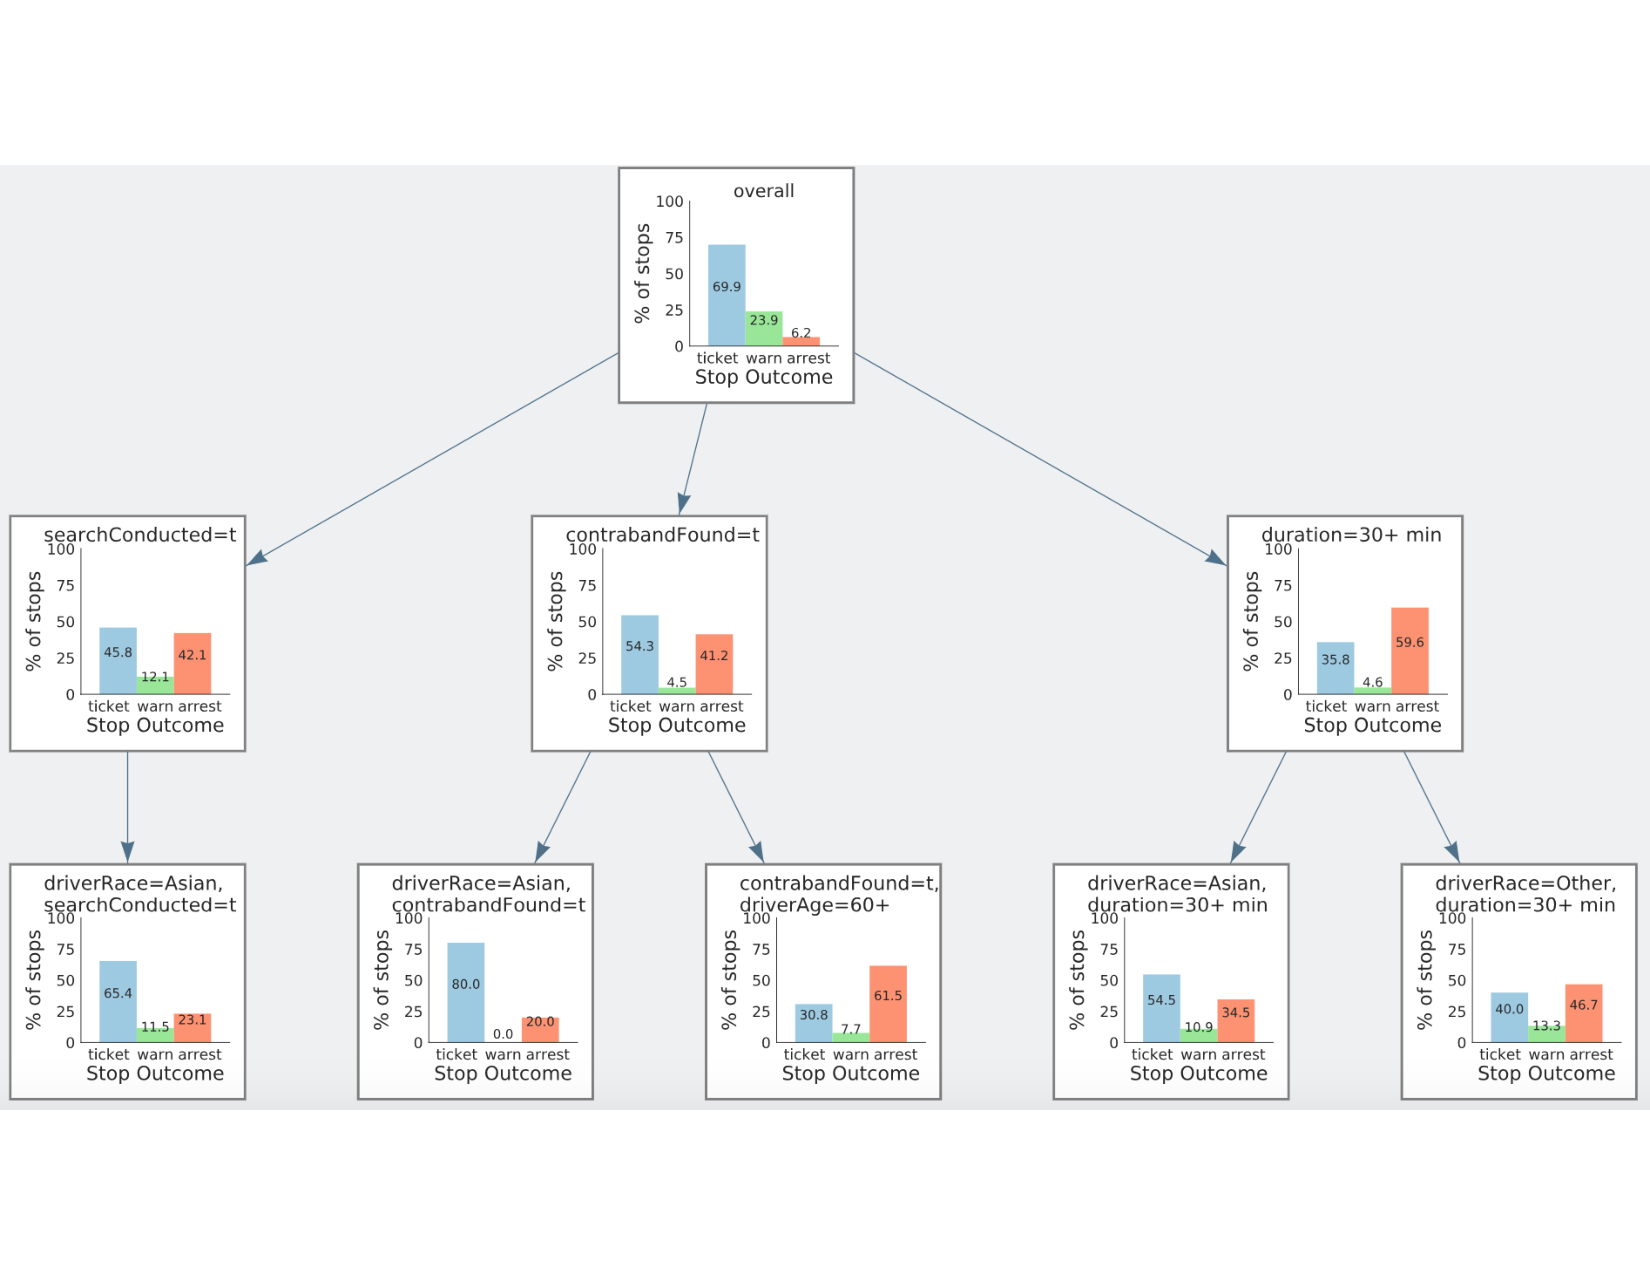
\includegraphics[width=\linewidth]{figs/storyboard.pdf}
\caption{Example dashboard generated by \sbd summarizing the key insights in the Police dataset.}
\label{fig:sbd}
\vspace{-10pt}
\end{wrapfigure} 

\par The effectiveness of \sbd largely 
comes from how the summary visualizations 
help users become more distributionally aware of the dataset. 
We define \emph{distribution awareness} 
as the aspect of data understanding in which users make sense of the key distributions across different data subsets and their relationships in the context of the dataset. With distribution awareness, 
even though it may be infeasible for an 
user to examine all possible data subsets, 
the user will still be able to draw meaningful 
insights and establish correlations 
about related visualizations by 
generalizing their understanding based 
on the limited number of visualizations
 presented in the dashboard. 
 Our evaluation study shows that facilitating 
 distribution awareness through \sbd 
 guides users to make better predictions 
 regarding unseen visualizations, 
 ranking attribute importance, and 
 retrieval of interesting visualizations 
 compared to dashboards generated from the baselines. 

\subsection{Research Challenges within the Minimal Setting: Distributional to Contextual Awareness}

\par The main research challenge that we aim to address in the minimal setting is the following: {\em How can contextual information be used to help facilitate better understanding, and guide users towards more informative next steps in their analysis?} The notion of distribution awareness is useful when considering the scenario at one static point in time of the analysis, such as during cold-start. In this section, we introduce a complementary notion of data understanding called \textit{contextual awareness}, which is essential when considering a dynamic analytic workflow for visual data exploration.
 
\par Contextual awareness is the aspect of 
data understanding related to 
the \textit{situation} (what is the information 
that I'm currently looking at and how did it come about?) 
and \textit{history} (what have I explored in the past 
and where should I look next?) of exploration. 
Situational understanding involves recognizing 
what data is in the current 
scope of analysis, 
including making sense of the data attributes 
and schema and keeping track of what filters or 
transformations have been applied to the displayed data. 
Historical understanding is associated with 
the user's past analysis actions on the data. 
As an example, an user may be interested 
in how the sales price of a product changes 
as a function of other dimensions variables, 
such as geographic location, year sold, and product type. 
Situational information informs them that they are 
looking at a bar chart with \textsc{x=TYPE}, \textsc{y=AVG(PRICE)}, 
whereas historical information points 
to the fact that they should explore the 
geographic dimension, since they have 
already explored the temporal attribute \textsc{YEAR}.

\par While the problem of data provenance 
has been well studied in database literature~\cite{Buneman2006,Cui2003,Woodruff1997}, the effects of showing provenance information 
to users during data analysis is an important but underexplored area. 
Moreover, within a dataset, history is essential 
in helping users navigate through the space 
of possible analysis actions and provide users 
with sense of coverage and completion. 
The notion of adding navigational cues 
to guide exploration in visual information spaces 
was first proposed in Willet et al.'s work on \textit{scented widgets}~\cite{Willett2007}. In Pirolli and Card's theory of information foraging, 
scents are cues that signifies the perceived benefit 
that one would receive during a search. 
Scented widgets adds to existing search interfaces 
by embedding visualizations that provide informational scents, 
such as histogram distributions of how popular a particular value is among users or using color to encode the size of a dataset in a drop-down menu. 
Recently, Sarvghad et al. have extended the idea 
of scented widgets to incorporate dimension coverage 
information during data exploration, 
including which dimensions have been explored so far, 
in what frequency, and in which combinations~\cite{Sarvghad2017}. 
Their study shows that visualizing dimension coverage 
leads to increased number of questions formulated, findings, and broader exploration. Interpretable and non-disruptive cues that enables 
users to visualize provenance and history help sustain contextual awareness and guide users towards 
more informative next steps in their analysis.%than participants who had no access to coverage information
\par Mechanisms that facilitate distribution awareness 
for users can effectively couple with contextual awareness 
in dynamic exploration situations 
to help update the user's mental model 
on the current data context. 
For example, the representative and outlier patterns 
in \zv provides summaries of data in context. 
When a dataset is filtered, the representative trends 
are updated accordingly. By being aware of both the 
context and the distributions, the users becomes 
distributionally aware of how the typical patterns 
and trends of the distributions changes in a particular context. %(i.e. I'm only looking at data filtered with ....),an overview of typical trends for the data to be queried.
\par We envision that by incorporating contextual 
information along with improving the recommendation (`pull') 
aspects of the \vidaql discovery modules, 
\vida will be well-equipped with the necessary 
information for making `active' recommendations. 
Contrary to `static' recommendations in \sbd and \seedb, 
where users need to submit some minimal required 
information to explicitly request 
for recommendations and the system 
performs only one type of recommendation, 
these next-generation systems 
actively seek for opportunities to 
provide appropriate recommendations 
that would be useful to the user at the 
specific stage of analysis by intelligently 
adapting the modes of recommendation 
to the context of user's analysis. 
This shift from static to active recommendation is analogical to the shift from precise to fuzzy querying in Section~\ref{sec:vague}, where the onus is more on the system to `guess' at the users intent. 
In active recommendations, instead of providing 
minimal information to request recommendation, 
the system will automatically infer implicit 
signals through other modalities of interaction. 
\vida can make use of this information to 
make better recommendations that can guide users 
towards meaningful stories and insights for further investigation.

\section{Concluding Remarks\label{sec:conclusion}}
\par Data is inherently agnostic to the diverse information needs that any particular user may have. 
Visual data exploration systems can 
help bridge the gap between what users want to 
get from the data through querying and 
what insights the data has to offer through recommendations. 
To facilitate a more productive collaboration, 
in this paper, we outline our vision for \vida, motivated by related work 
from precise visual querying of informative visualizations 
to accelerate the process of data discovery; 
to interpreting ambiguous and high-level queries 
through query refinement feedback; to recommendations that promote better distributional 
and contextual awareness for users. 
We hope that the agenda sketched out in this paper 
sheds light on the many more exciting research 
questions and opportunities 
to come in this nascent field.


{\footnotesize \bibliographystyle{named}
\begin{thebibliography}{}

\bibitem[\protect\citeauthoryear{Abouzied \bgroup \em et al.\egroup
  }{2012}]{Abouzied2012}
Azza Abouzied, J~Hellerstein, and A~Silberschatz.
\newblock {Dataplay: interactive tweaking and example-driven correction of
  graphical database queries}.
\newblock {\em Proceedings of the 25th annual ACM symposium on User interface
  software and technology}, pages 207--217, 2012.

\bibitem[\protect\citeauthoryear{Amar \bgroup \em et al.\egroup
  }{2005}]{Amar2005}
Robert Amar, James Eagan, and John Stasko.
\newblock {Low-level components of analytic activity in information
  visualization}.
\newblock {\em Proceedings - IEEE Symposium on Information Visualization, INFO
  VIS}, pages 111--117, 2005.

\bibitem[\protect\citeauthoryear{Anand and Talbot}{2015}]{Anand2015}
Anushka Anand and Justin Talbot.
\newblock {Automatic Selection of Partitioning Variables for Small Multiple
  Displays}.
\newblock {\em IEEE Transactions on Visualization and Computer Graphics},
  22(1):669 -- 677, 2015.

\bibitem[\protect\citeauthoryear{Buneman \bgroup \em et al.\egroup
  }{2006}]{Buneman2006}
Peter Buneman, Adriane Chapman, and James Cheney.
\newblock Provenance management in curated databases.
\newblock In {\em Proceedings of the 2006 ACM SIGMOD International Conference
  on Management of Data}, SIGMOD '06, pages 539--550, New York, NY, USA, 2006.
  ACM.

\bibitem[\protect\citeauthoryear{Correll and
  Gleicher}{2016}]{correll2016semantics}
Michael Correll and Michael Gleicher.
\newblock The semantics of sketch: Flexibility in visual query systems for time
  series data.
\newblock In {\em Visual Analytics Science and Technology (VAST), 2016 IEEE
  Conference on}, pages 131--140. IEEE, 2016.

\bibitem[\protect\citeauthoryear{Cui and Widom}{2003}]{Cui2003}
Y.~Cui and J.~Widom.
\newblock Lineage tracing for general data warehouse transformations.
\newblock {\em Proceedings of the VLDB Endowment}, 12(1):41--58, May 2003.

\bibitem[\protect\citeauthoryear{{Drlica Wagner et
  al.}}{2018}]{Drlica-Wagner2017}
{Drlica Wagner et al.}
\newblock Dark energy survey year 1 results: The photometric data set for
  cosmology.
\newblock {\em The Astrophysical Journal Supplement Series}, 235(2):33, 2018.

\bibitem[\protect\citeauthoryear{Embley}{1989}]{Embley1989}
David~W. Embley.
\newblock Nfql: The natural forms query language.
\newblock {\em ACM Transactions on Database Systems (TODS)}, 14(2):168--211,
  June 1989.

\bibitem[\protect\citeauthoryear{Fast \bgroup \em et al.\egroup
  }{2018}]{Fast2018}
Ethan Fast, Binbin Chen, Julia Mendelsohn, Jonathan Bassen, and Michael~S.
  Bernstein.
\newblock Iris: A conversational agent for complex tasks.
\newblock In {\em Proceedings of the 2018 CHI Conference on Human Factors in
  Computing Systems}, CHI '18, pages 473:1--473:12, New York, NY, USA, 2018.
  ACM.

\bibitem[\protect\citeauthoryear{Gao \bgroup \em et al.\egroup
  }{2015}]{Gao2015}
Tong Gao, Mira Dontcheva, Eytan Adar, Zhicheng Liu, and Karrie~G. Karahalios.
\newblock Datatone: Managing ambiguity in natural language interfaces for data
  visualization.
\newblock In {\em Proceedings of the 28th Annual ACM Symposium on User
  Interface Software \&\#38; Technology}, UIST '15, pages 489--500, New York,
  NY, USA, 2015. ACM.

\bibitem[\protect\citeauthoryear{Heer and Shneiderman}{2012}]{Heer2012}
Jeffrey Heer and Ben Shneiderman.
\newblock {Interactive Dynamics for Visual Analysis}.
\newblock {\em ACM Queue}, 10(2):30, 2012.

\bibitem[\protect\citeauthoryear{Hochheiser and
  Shneiderman}{2004}]{hochheiser2004dynamic}
Harry Hochheiser and Ben Shneiderman.
\newblock Dynamic query tools for time series data sets: timebox widgets for
  interactive exploration.
\newblock {\em Information Visualization}, 3(1):1--18, 2004.

\bibitem[\protect\citeauthoryear{Hoque \bgroup \em et al.\egroup
  }{2017}]{Hoque2017}
Enamul Hoque, Vidya Setlur, Melanie Tory, and Isaac Dykeman.
\newblock {Applying Pragmatics Principles for Interaction with Visual
  Analytics}.
\newblock {\em IEEE Transactions on Visualization and Computer Graphics}, (c),
  2017.

\bibitem[\protect\citeauthoryear{Jagadish \bgroup \em et al.\egroup
  }{2007}]{Jagadish2007}
H.~V. Jagadish, Adriane Chapman, Aaron Elkiss, Magesh Jayapandian, Yunyao Li,
  Arnab Nandi, and Cong Yu.
\newblock Making database systems usable.
\newblock SIGMOD '07, pages 13--24, New York, NY, USA, 2007. ACM.

\bibitem[\protect\citeauthoryear{Kandel \bgroup \em et al.\egroup
  }{2012}]{Kandel2012}
Sean Kandel, Ravi Parikh, Andreas Paepcke, Joseph Hellerstein, and Jeffrey
  Heer.
\newblock Profiler: Integrated statistical analysis and visualization for data
  quality assessment.
\newblock In {\em Advanced Visual Interfaces}, 2012.

\bibitem[\protect\citeauthoryear{Khoussainova \bgroup \em et al.\egroup
  }{2010}]{Khoussainova2010}
Nodira Khoussainova, YongChul Kwon, Magdalena Balazinska, and Dan Suciu.
\newblock {Snipsuggest: Context-aware autocompletion for sql}.
\newblock {\em Proceedings of the VLDB Endowment}, 4(1):22--33, 2010.

\bibitem[\protect\citeauthoryear{Lee \bgroup \em et al.\egroup }{}]{Lee2018}
Doris~Jung{-}Lin Lee, Himel Dev, Huizi Hu, Hazem Elmeleegy, and Aditya~G.
  Parameswaran.
\newblock Storyboard: Navigating through data slices with distributional
  awareness.

\bibitem[\protect\citeauthoryear{Lee \bgroup \em et al.\egroup
  }{2017}]{Lee2017}
Doris~Jung{-}Lin Lee, John Lee, Tarique Siddiqui, Jaewoo Kim, Karrie
  Karahalios, and Aditya~G. Parameswaran.
\newblock Accelerating scientific data exploration via visual query systems.
\newblock {\em CoRR}, abs/1710.00763, 2017.

\bibitem[\protect\citeauthoryear{Mannino and Abouzied}{2018}]{Mannino2018}
Miro Mannino and Azza Abouzied.
\newblock Expressive time series querying with hand-drawn scale-free sketches.
\newblock In {\em Proceedings of the 2018 CHI Conference on Human Factors in
  Computing Systems}, CHI '18, pages 388:1--388:13, New York, NY, USA, 2018.
  ACM.

\bibitem[\protect\citeauthoryear{Meliou \bgroup \em et al.\egroup
  }{2010}]{meliou2010causality}
Alexandra Meliou, Wolfgang Gatterbauer, Joseph~Y Halpern, Christoph Koch,
  Katherine~F Moore, and Dan Suciu.
\newblock Causality in databases.
\newblock {\em IEEE Data Engineering Bulletin}, 33(EPFL-ARTICLE-165841):59--67,
  2010.

\bibitem[\protect\citeauthoryear{{Mohebbi et al.}}{2011}]{mohebbi2011google}
{Mohebbi et al.}
\newblock Google correlate whitepaper.
\newblock 2011.

\bibitem[\protect\citeauthoryear{Morton \bgroup \em et al.\egroup
  }{2014}]{Morton2014}
Kristi Morton, Magdalena Balazinska, Dan Grossman, and Jock Mackinlay.
\newblock {Support the Data Enthusiast: Challenges for Next-Generation
  Data-Analysis Systems}.
\newblock {\em Proceedings of the VLDB Endowment, Volume 7, pp. 453–456,
  2014}, 7:453--456, 2014.

\bibitem[\protect\citeauthoryear{Nandi \bgroup \em et al.\egroup
  }{2013}]{Nandi2013}
Arnab Nandi, Lilong Jiang, and Michael Mandel.
\newblock {Gestural query specification}.
\newblock {\em Proceedings of the VLDB Endowment}, 7(4):289--300, 2013.

\bibitem[\protect\citeauthoryear{Olston and Chi}{2003}]{Olston2003}
Christopher Olston and Ed~Chi.
\newblock {ScentTrails: Integrating browsing and searching on the Web}.
\newblock {\em ACM Transactions on Computer Human Interaction TOCHI},
  10(3):177--197, 2003.

\bibitem[\protect\citeauthoryear{Pierson \bgroup \em et al.\egroup
  }{2017}]{police}
E.~Pierson, C.~Simoiu, J.~Overgoor, S.~Corbett-Davies, V.~Ramachandran,
  C.~Phillips, and S.~Goel.
\newblock A large-scale analysis of racial disparities in police stops across
  the united states, 2017.

\bibitem[\protect\citeauthoryear{Roy and Suciu}{2014}]{roy2014formal}
Sudeepa Roy and Dan Suciu.
\newblock A formal approach to finding explanations for database queries.
\newblock In {\em Proceedings of the 2014 ACM SIGMOD international conference
  on Management of data}, pages 1579--1590. ACM, 2014.

\bibitem[\protect\citeauthoryear{Sarawagi \bgroup \em et al.\egroup
  }{1998}]{Sarawagi1998}
Sunita Sarawagi, Rakesh Agrawal, and Nimrod Megiddo.
\newblock Discovery-driven exploration of olap data cubes.
\newblock EDBT '98, pages 168--182, Berlin, Heidelberg, 1998. Springer-Verlag.

\bibitem[\protect\citeauthoryear{Sarawagi}{2000}]{Sarawagi2000}
S.~Sarawagi.
\newblock {User-adaptive exploration of multidimensional data}.
\newblock {\em Proceedings of the VLDB Endowment}, pages 307--316, 2000.

\bibitem[\protect\citeauthoryear{Sarvghad \bgroup \em et al.\egroup
  }{2017}]{Sarvghad2017}
Ali Sarvghad, Melanie Tory, and Narges Mahyar.
\newblock {Visualizing Dimension Coverage to Support Exploratory Analysis}.
\newblock {\em IEEE Transactions on Visualization and Computer Graphics},
  23(1):21--30, 2017.

\bibitem[\protect\citeauthoryear{Setlur \bgroup \em et al.\egroup
  }{2016}]{Setlur2016}
Vidya Setlur, Sarah~E Battersby, Melanie Tory, Rich Gossweiler, and Angel~X
  Chang.
\newblock {Eviza: A Natural Language Interface for Visual Analysis}.
\newblock {\em Proceedings of the 29th Annual Symposium on User Interface
  Software and Technology - UIST '16}, pages 365--377, 2016.

\bibitem[\protect\citeauthoryear{Siddiqui \bgroup \em et al.\egroup
  }{2016}]{Siddiqui2016}
Tarique Siddiqui, Albert Kim, John Lee, Karrie Karahalios, and Aditya
  Parameswaran.
\newblock Effortless data exploration with zenvisage: An expressive and
  interactive visual analytics system.
\newblock {\em Proceedings of the VLDB Endowment}, 10(4):457--468, November
  2016.

\bibitem[\protect\citeauthoryear{Siddiqui \bgroup \em et al.\egroup
  }{2019}]{Siddiqui2018}
Tarique Siddiqui, Paul Luh, Zesheng Wang, Karrie Karahalios, and Aditya~G.
  Parameswaran.
\newblock Shapesearch: Flexible pattern-based querying of trend line
  visualizations.
\newblock {\em Proceedings of the VLDB Endowment}, 2019.

\bibitem[\protect\citeauthoryear{Stolte \bgroup \em et al.\egroup
  }{2002}]{Stolte2002}
C.~Stolte, D.~Tang, and P.~Hanrahan.
\newblock {Polaris: a system for query, analysis, and visualization of
  multidimensional relational databases}.
\newblock {\em IEEE Transactions on Visualization and Computer Graphics},
  8(1):1--14, 2002.

\bibitem[\protect\citeauthoryear{Vartak \bgroup \em et al.\egroup
  }{2015}]{Vartak2015}
Manasi Vartak, Samuel Madden, and Aditya~N Parmeswaran.
\newblock {SEEDB : Supporting Visual Analytics with Data-Driven
  Recommendations}.
\newblock {\em Proceedings of the VLDB Endowment, Volume 8, No. 13, 2015},
  2015.

\bibitem[\protect\citeauthoryear{Vartak \bgroup \em et al.\egroup
  }{2017}]{Vartak2017}
Manasi Vartak, Silu Huang, Tarique Siddiqui, Samuel Madden, and Aditya
  Parameswaran.
\newblock {Towards Visualization Recommendation Systems}.
\newblock {\em ACM SIGMOD Record}, 45(4):34--39, 2017.

\bibitem[\protect\citeauthoryear{Wattenberg}{2001}]{wattenberg2001sketching}
Martin Wattenberg.
\newblock Sketching a graph to query a time-series database.
\newblock In {\em CHI'01 Extended Abstracts on Human factors in Computing
  Systems}, pages 381--382. ACM, 2001.

\bibitem[\protect\citeauthoryear{Wilkinson}{2005}]{Wilkinson2005}
Leland Wilkinson.
\newblock {\em The Grammar of Graphics (Statistics and Computing)}.
\newblock Springer-Verlag, Berlin, Heidelberg, 2005.

\bibitem[\protect\citeauthoryear{Willett \bgroup \em et al.\egroup
  }{2007}]{Willett2007}
Wesley Willett, Jeffrey Heer, and Maneesh Agrawala.
\newblock {Scented widgets: Improving navigation cues with embedded
  visualizations}.
\newblock {\em IEEE Transactions on Visualization and Computer Graphics},
  13(6):1129--1136, 2007.

\bibitem[\protect\citeauthoryear{Wongsuphasawat \bgroup \em et al.\egroup
  }{2017}]{Wongsuphasawat2017}
Kanit Wongsuphasawat, Zening Qu, Dominik Moritz, Riley Chang, Felix Ouk,
  Anushka Anand, Jock Mackinlay, Bill Howe, and Jeffrey Heer.
\newblock Voyager 2: Augmenting visual analysis with partial view
  specifications.
\newblock In {\em ACM Human Factors in Computing Systems (CHI)}, 2017.

\bibitem[\protect\citeauthoryear{Woodruff and Stonebraker}{1997}]{Woodruff1997}
Allison Woodruff and Michael Stonebraker.
\newblock Supporting fine-grained data lineage in a database visualization
  environment.
\newblock In {\em Proceedings of the Thirteenth International Conference on
  Data Engineering}, ICDE '97, pages 91--102, Washington, DC, USA, 1997. IEEE
  Computer Society.

\bibitem[\protect\citeauthoryear{Wu and Madden}{2013}]{Wu2013}
Eugene Wu and Samuel Madden.
\newblock {Scorpion: Explaining Away Outliers in Aggregate Queries}.
\newblock {\em Proceedings of the VLDB Endowment}, 6(8):553--564, 2013.

\bibitem[\protect\citeauthoryear{Zgraggen \bgroup \em et al.\egroup
  }{2015}]{Zgraggen2015}
Emanuel Zgraggen, Steven~M Drucker, Danyel Fisher, and Robert DeLine.
\newblock {(s|qu)eries: Visual Regular Expressions for Querying and Exploring
  Event Sequences}.
\newblock {\em Proceedings of the 33rd Annual ACM Conference on Human Factors
  in Computing Systems}, pages 2683--2692, 2015.

\bibitem[\protect\citeauthoryear{Zloof}{1975}]{Zloof1975}
Moshe~M Zloof.
\newblock {Query by Example}.
\newblock {\em National Computer Conference}, pages 431--438, 1975.

\end{thebibliography}
}
\end{document}

